\chapter{Redes de Sensores Sem Fio}

Graças aos avanços tecnológicos na área de comunicação sem fio e de eletrônicos tem sido cada vez mais fácil desenvolver nós sensores multifuncionais de baixo custo e consumo de energia capazes de se comunicar a curtas distâncias. Disso surge a ideia da criação de redes de sensores sem fio.

Redes de sensores sem fio(RSSF) são redes compostas por um grande número de nós sensores densamente distribuídos dentro de um fenômeno ou próximo a ele, cujas posições não precisam ser predeterminadas e que trabalham de forma cooperativa para a realização de tarefas. Isso possibilita a distribuição aleatória em regiões inacessíveis, porém também torna necessária a criação de protocolos e algoritmos com capacidade de auto organização\cite{Akyildiz2002}.

\begin{figure}[!htb]
\centering
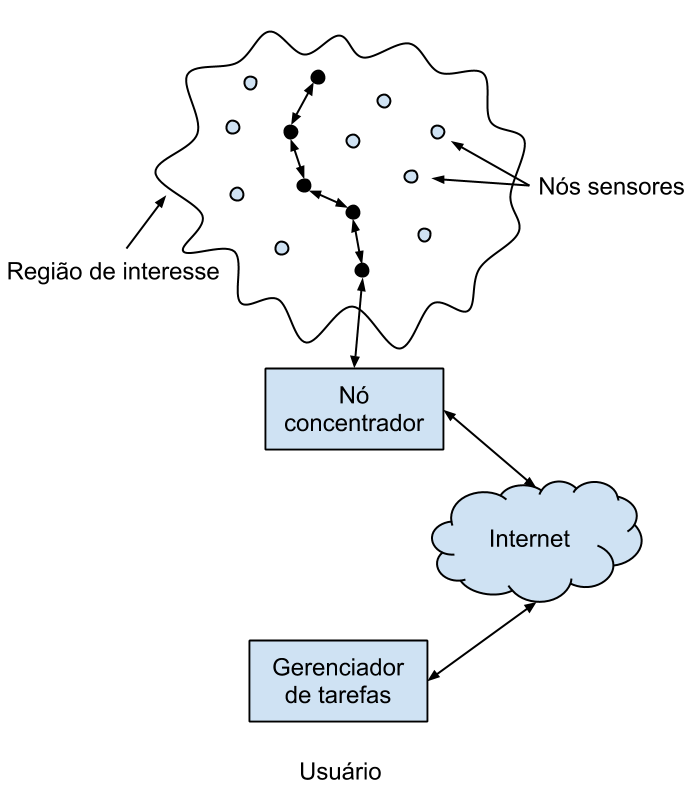
\includegraphics[width=200px,height=280px]{./Pictures/SensorNodesScatteredInASensorField.png}
% SensorNodesScatteredInASensorField.png: 816x1056 pixel, 96dpi, 21.59x27.94 cm, bb=0 0 612 792
% pdfLaTeX aceita figuras no formato PNG, JPG ou PDF
% figuras vetoriais podem ser exportadas para eps e depois convertidas para pdf usando epstopdf
\caption{Exemplo da distribuição dos nós de uma RSSF em uma região de interesse} %legenda
\label{fig:snsf} %rotulo para refencia
\end{figure}

A Figura~\ref{fig:snsf} mostra como os nós de uma rede de sensores ficam distribuídos em uma região de interesse(\textit{sensor field}). Cada um dos nós(\textit{sensor nodes}) coleta dados do ambiente e pode roteá-los até o nó \textit{sink} (nó que reúne as informações da rede) e este pode comunicar-se com o gerenciador de tarefas por meio da internet ou de satélites.

Romer e Matter(2004)\cite{Romer2004} definem RSSF como redes \textit{ad hoc} de larga escala, \textit{multi-hop}, não particionada composta por nós sensores, em sua maioria imóveis, largamente homogêneos, pequenos e com recursos limitados, randomicamente distribuídos em uma área de interesse.

Karl e Willing(2005)\cite{Karl2005} apresentam uma definição de redes \textit{ad hoc} como redes configuradas para, literalmente, atender a um propósito específico e a necessidades específicas de comunicação. \cite{Karl2005} apresenta também uma definição para \textit{Mobile Ad Hoc Networks}(MANET) que seria uma rede \textit{ad hoc} associada à comunicação sem fio(\textit{wireless}) e à mobilidade dos nós participantes. 


Listadas abixo estão algumas diferenças significativas entre redes \textit{ad hoc} e RSSF:
\begin{itemize} 
	\item O número de nós sensores em RSSF pode ser de uma ordem de magnitude muio acima da encontrada em redes \textit{ad hoc}\cite{Akyildiz2002}.
	\item MANET são utilizadas em aplicações como comunicação por voz ou acesso a infraestrutura remota necessitando assim de equipamentos robustos o suficiente para suportar esse tipo de aplicações ao contrário de RSSFs que são compostas por equipamentos bem mais simples e limitados\cite{Karl2005}. 
	\item RSSF são capazes de comportar variados cenários de aplicação, devido ao grande número de combinações possíveis de tecnologias de comunicação, computação e sensores. Por exemplo conseguindo trabalhar em diversas e variáveis densidades, o que irá requerer o uso de diferentes protocolos ou protocolos adaptativos. Tal flexibilidade existe também em MANET, porém em um nível bastante reduzido\cite{Karl2005}. 
	\item A densidade das RSSF é bem maior que a encontrada nas MANET\cite{Akyildiz2002}.
	\item Nós sensores de uma RSSF são suscetíveis a erros e a topologia da rede muda com frequência\cite{Akyildiz2002}. 
	\item Em RSSF predomina o paradigma de comunicação \textit{broadcast}, ao contrário do que predomina em redes \textit{ad hoc} que é a comunicação \textit{point-to-point}.
	\item Nós de uma RSSF podem não possuir uma identificação global devido ao grande número de nós sensores, pois isso causaria um grande \textit{overhead}.
\end{itemize} 

% +++++++++++++++++++++++++++++++++++++++++++++++++++++++++++++++++++++++++++++++++++++++++++++++++++++++++++++++++++++
\section{Características de RSSF} \label{sec:featuresRSSF}
% +++++++++++++++++++++++++++++++++++++++++++++++++++++++++++++++++++++++++++++++++++++++++++++++++++++++++++++++++++++

Há inúmeros problemas encontrados nesse tipo de redes e um número igualmente grande de soluções propostas para cada um desses problemas. De maneira geral, nós de uma rede de sensores sem fio são alimentados por baterias e, consequentemente, possuem um tempo de vida útil consideravelmente limitado, tendo em vista que, na maioria das utilizações desse tipo de rede não é possível fazer a substituição das baterias. Tal asserção baseia-se no fato que esse tipo de solução, dadas as suas limitações, só seria empregada em casos onde outras soluções mais simples ou eficientes não pudessem ser empregadas, como no monitoramento de áreas de difícil acesso, por exemplo, o interior de florestas ou áreas de desastre. 

Algumas das principais características que uma RSSF deve apresentar são:
 \begin{itemize}
 \item \textbf{Tolerância a falhas:} Alguns nós da rede podem deixar de funcionar devido a vários fatores como o fim de suas baterias ou dano físico. Tolerância a falhas é a capacidade de manter a rede de sensores funcionando sem interrupções devido a falhas em nós sensores\cite{Srisathapornphat2001,Hoblos2000}.
 \item \textbf{Escalabilidade:} O número de nós distribuídos para o estudo de um fenômeno pode atingir valores muito elevados(ordem de centenas de milhares ou mais). Além disso pode existir um número muito grande de nós em uma área muito pequena(alta densidade). Devem ser desenvolvidos mecanismos e protocolos capazes de trabalhar com esse número de nós.
 \item \textbf{Tempo de vida:} Na maioria dos cenários de utilização de RSSF limitam ou impossibilitam a substituição de baterias nos nós\cite{Karl2005}. Ainda assim, espera-se que uma rede de sensores permaneça em funcionamento por um determinado período de tempo necessário à realização de uma missão ou o maior tempo possível. Portanto, torna-se evidente a necessidade de fazer com que a rede opere de modo eficiente em relação ao consumo de energia.
 \item \textbf{Programabilidade:} Os nós de uma rede de sensores devem processar informações, mas além disso precisam ser capazes de se adaptar a mudanças em suas tarefas. Eles devem ser programáveis e sua programação deve ser passível de alterações mesmo quando em operação para atender a novas tarefas que venham a se tornar importantes\cite{Karl2005}.
 \item \textbf{Manutenibilidade:} Com o passar do tempo podem ocorrer mudanças tanto no ambiente como na rede de sensores. Essas mudanças podem ser causadas por vários fatores, como falha de nós ou surgimento de novas tarefas. A rede deve adaptar-se a essas mudanças e monitorar o seu próprio estado, fazendo as alterações nos parâmetros operacionais quando necessário, por exemplo reduzindo a qualidade do serviço quando o nível de energia estiver baixo. Ela poderia interagir com mecanismos externos de manutenção para garantir a continuidade de sua operação a um nível mínimo de qualidade necessário por uma maior período de tempo\cite{Mainwaring2002}.
 \end{itemize}

%=====================================================================
\section{Protocolos em RSSF} 
%==============================

A pilha de protocolos usados em redes de sensores sem fio são responsáveis por prover comunicação eficiente, em termos de energia e roteamento, no meio sem fio, integração entre dados e protocolos de rede e promover o esforço cooperativo dos nós sensores \cite{Akyildiz2002}. Os protocolos estão distribuídos entre as camadas da rede. Uma descrição de cada camada é apresentada em \cite{Akyildiz2002} e descrita resumidamente a seguir. A Figura~\ref{fig:protocolStack} é uma representação da pilha de protocolos.

\begin{figure}[!htb]
\centering
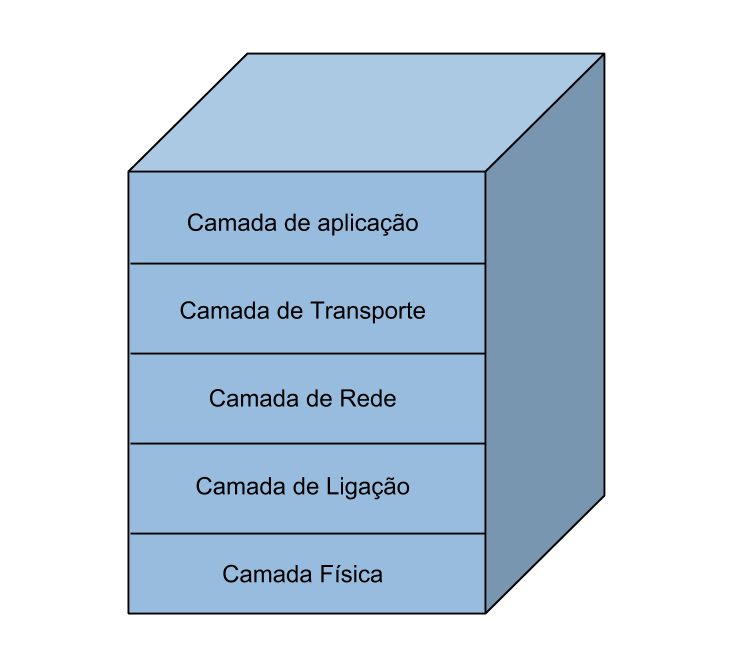
\includegraphics[width=230px,height=280px]{./Pictures/ProtocolStack.png}
% SensorNodesScatteredInASensorField.png: 816x1056 pixel, 96dpi, 21.59x27.94 cm, bb=0 0 612 792
% pdfLaTeX aceita figuras no formato PNG, JPG ou PDF
% figuras vetoriais podem ser exportadas para eps e depois convertidas para pdf usando epstopdf
\caption{Pilha de protocolos em redes de sensores sem fio} %legenda
\label{fig:protocolStack} %rotulo para refencia
\end{figure}


 %---------------------------------------------------------------------
 \subsection{Camada física (\textit{physical layer})} 
 %------------------------------------------------------

 A camada física é responsável por selecionar a frequência, geração de frequência portadora\textit{carrier frequency generation}, detecção de sinais, modulação e encriptação de dados. O custo, tanto em termos de consumo de energia quanto em complexidade de implementação, da comunicação sem fio a longas distâncias é muito elevado. Em redes de sensores sem fio, a minimização do consumo de energia tem importância significativa na propagação e nos efeitos que causam desvanecimento do sinal. Em geral, a potência necessária para transmitir um sinal a uma distância \textit{$d$} é diretamente proporcional a \textit{$d^{n}$}, sendo 2 <= \textit{n} < 4. n é próximo de 4 para antenas muito baixas e canais muito próximas do chão \cite{Pottie2000} citado por \cite{Akyildiz2002}.
 
 %---------------------------------------------------------------------
 \subsection{Camada de ligação de dados(\textit{Data Link Layer}) }
 %--------------------------------------------------------------------
 
 Camada de ligação de dados é a camada responsável por multiplexação de fluxos de dados(\textit{data streams}), detecção de quadros de dados(\textit{data frames}), acesso ao meio(\textit{medium access}) e controle de erros(\textit{error control}).
 
 \subsubsection{Protocolos de controle de acesso ao meio}
 
 Protocolos de controle de acesso ao meio (\textit{Medium Access Control Protocols}) atuam nessa camada. Eles coordenam o acesso ao meio físico por nós ativos. Esses protocolos são de grande importância, uma vez que o canal de comunicação sem fio (\textit{wireless}) é inerentemente propenso a erros, além de outros problemas específicos desse tipo de rede, tais como: o problema do terminal escondido (\textit{hidden-terminal}), problema do terminal exposto(\textit{exposed-terminal}) e efeitos do desvanecimento de sinal (\textit{signal fading effects}) Kumar et. al. (2006) \cite{Kumar06mediumaccess}. Esses protocolos serão abordados mais detalhadamente na sessão ~\ref{sec:macProtocols}.

 
 %---------------------------------------------------------------------
 \subsection{Camada de rede( \textit{Network layer})} 
 %------------------------------------------------------
 
 Técnicas convencionais de roteamento não são aplicáveis às características específicas desse tipo de redes (algumas delas podem ser encontradas na sessão ~\ref{sec:featuresRSSF}). A camada de rede em redes desenvolvida de acordo com as seguintes restrições \cite{Guerses2005}:
 
 \begin{itemize}
 \item \textbf{Não há um identificador global}, devido a existência de poucos dados de eventos e um grande número de nós.
 \item \textbf{Eficiência de energia} é necessária para aumentar o tempo de vida da rede.
 \item \textbf{Descoberta de rotas auto organizável} para lidar com mudanças na topologia da rede.
 \item \textbf{Modelo de distribuição de dados} pode ser dos tipos \cite{Tilak02ataxonomy}:
 \subitem \textbf{contínuo} - sensores entregam os dados continuamente;
 \subitem \textbf{dirigido a eventos} - sensores entregam dados ao detectarem um evento de interesse;
 \subitem \textbf{dirigido a consultas} - os nós entregam dados a partir da uma solicitação iniciada pelo observador;
 \item \textbf{Processamento em rede} por meio da utilização de ``funções de agregação'' é um requisito para comunicação eficiente em termos de energia;
 \item \textbf{Comunicação local inter sensor} é um requisito para aplicações, bem como para o processamento em rede;
 \item \textbf{Qualidade de serviço} (largura de banda, quantidade de erros e latência) deve atenter aos requisitos das aplicações; 
 
 \end{itemize}

 %---------------------------------------------------------------------
 \subsection{Camada de transporte} 
 %------------------------------------------------------
 
 Muitas aplicações de redes de sensores sem fio requerem mecanismos de controle de congestionamento para regular a quantidade de tráfego injetada na rede com o objetivo de evitar perda de pacotes e para atribuir confiabilidade à entrega de pacotes e eventos \cite{RaSaGu2008-InCol}. Em várias aplicações há nós responsáveis por capturar informações críticas e enviá-las a um nó concentrador (\textit{sink node}) \cite{RaSaGu2008-InCol}. Os protocolos dessa camada são desenvolvidos para atender a essas restrições e garantir que os pacotes sejam enviados e alcancem seus destinos corretamente.

 \subsection{Camada de aplicação}
 
 Segundo Alkyildniz et. al. (2002), embora haja muitas aplicações propostas para redes de sensores, potenciais protocolos para a camada de aplicação permanecem em uma região altamente inexplorada. Esses protocolos possibilitam a interação entre a camada de aplicação e as camadas inferiores. Há três protocolos mais comuns utilizados nessa camada. 
 
 \begin{itemize}
 \item \textbf{Protocolo de gerenciamento de sensores:} protocolos de gerenciamento na camada de aplicação tornam o \textit{hardware} e o \textit{software} das camadas inferiores transparentes para aplicações de gerenciamento de redes de sensores.
 \item \textbf{Protocolo de atribuição de tarefas e anúncio de dados (\textit{data advertisement}):} utilizado para atribuição de tarefas aos nós e também para comunicação de detecção de eventos pelos nós.
 \item \textbf{Protocolo de requisição (\textit{sensor query}) e disseminação de dados:} utilizados para fazer consultas ou requisições de dados aos sensores e devolução das respectivas respostas.
 \end{itemize}


\section{Controle de acesso ao meio}
\label{sec:macProtocols}

Protocolos de controle de acesso ao meio(MAC) são a primeira camada de protocolo acima da camada física e são responsáveis por prover endereçamento e acesso ao canal de comunicação. Segundo Karl and Willig(2005)\cite{Karl2005},a tarefa principal de qualquer protocolo MAC é regular o acesso de um número de nós a um meio de comunicação compartilhado, de tal modo que os requisitos de performance de cada aplicação sejam satisfeitos.

Nós sensores são alimentados por baterias, o que faz com que o consumo de energia seja uma restrição muito forte a ser tratada. Crescentes avanços tecnológicos tem tornado o custo de produção dos nós cada vez menor. Em razão disso, tem se tornado cada vez mais vantajoso substituir os nós ao invés de trocar suas baterias, tendo em vista que, na maioria dos casos, eles são inseridos em ambientes que dificultam ou mesmo impossibilitam o procedimento de troca. 

Segundo Ye (2002)\cite{Ye2002}, para desenvolver protocolos para redes de sensores, é preciso considerar como atributos principais a serem alcançados: eficiência no consumo de energia para aumentar a vida útil da rede, dado às dificuldades de substituição das baterias; escalabilidade para adaptação a mudanças no tamanho, densidade e topologia da rede, uma vez que alguns nós da rede irão morrer com o passar do tempo, novos nós podem ser inseridos na rede mais tarde, além disso, alguns nós podem se mover para locais diferentes. Outros atributos como justiça na distribuição de recursos(por exemplo o meio de comunicação), latência, e ritmo de transferência de dados que são tidos como principais em outros tipos de redes sem fio são aqui tidos como secundários.

%---------------------------------------------------------------------
\subsection{Padrões de comunicação em RSSFs}
\label{sec:comnPatt}
%-------------------------------------------
 
Segundo Demirkol et. al.(2006) \cite{Demirkol2006}, os tipos de padrões de comunicação em RSSFs determinam o comportamento do tráfego de dados na redes de sensores que deve ser tratado pelos protocolos de controle de acesso ao meio(MAC). 

Kulkarni (2004)\cite{Kulkarni2004} define três tipos de comunicação em redes de sensores sem fio: \textit{broadcast}, \textit{convergecast}, \textit{local gossip}. O padrão \textit{broadcast} é geralmente utilizados por estações base (\textit{sink nodes}) para trasmitir informações para todos os nós da rede. Pacotes enviados em \textit{broadcast} podem conter requisições por informações dos sensores, atualizações do programa para os nós sensores, pacotes de controle para todo o sistema, etc. \textit{Local gossip} ocorre quando um nó sensor detecta um evento e o comunica a cada um de seus vizinhos localmente (dentro do alcance de seu radiotransmissor). Após um grupo de nós detectar um evento, é necessário comunicá-lo ao centro de informações, esse padrão de comunicação é chamado \textit{convergecast} (quando um grupo de sensores se comunica com um sensor específico).

%---------------------------------------------------------------------
\subsection{Classificação de Protocolos de Controle de Acesso ao Meio}
%---------------------------------------------------------------------

A cada dia surgem novas propostas de protocolos MAC que utilizam diferentes técnicas para alcançar melhores resultados em termos de consumo de energia, latência, qualidade de serviço, etc., de acordo com as necessidades de cada aplicação. Chandra \cite{Chandra_2wireless} classifica os protocolos MAC nas seguintes classes: protocolos de atribuição fixa, protocolos de atribuição por demanda e protocolos de acesso aleatório.

 \subsubsection{Protocolos de atribuição fixa} 
 
 Cada nó recebe uma porção do recursos por um período de tempo considerado longo (da ordem de minutos, horas, ou mesmo maior) e pode utilizá-los de maneira exclusiva naquele período de tempo, ou seja, somente o nó ao qual um recurso foi atribuído pode acessar esse recurso no espaço de tempo que foi para ele reservado. 
 
 A atribuição desses recursos não é feita de maneira permanente devido à necessidade de adaptação a possíveis alterações na topologia da rede (quando ocorre a morte, inserção ou movimentação de nós na rede, por exemplo). Esse tipo de atribuição feito por períodos consideravelmente longos pode causar efeitos negativos à característica de escalabilidade da rede. 
 
 Como exemplos desse tipo de protocolo tem-se o \textit{Time Divided Multiple Access} (TDMA) \cite{Kulkarni2004} onde o tempo de uso dos recursos é dividido em \textit{slots} que são atribuídos aos nós da rede, \textit{Frequency Division Multiple Access} (FDMA) onde a banda de frequência e dividida em vários sub-canais (faixas de frequência) que são atribuídos aos nós da rede \cite{Arms_frequencyagile}.
	
 \subsubsection{Protocolos de atribuição por demanda} 
 
 Nesse tipo de protocolo, ao contrário dos protocolos de atribuição fixa, os recursos são distribuídos entre os nós por um período de tempo relativamente curto (da ordem de dezenas de milissegundos), geralmente o tempo necessário para o envio de um conjunto de pacotes de dados. Caso um nó necessite utilizar algum recurso, este deve fazer uma solicitação a um nó central que seja responsável por coordenar o uso de tal recurso, que por sua vez retorna a confirmação ou não da alocação do recurso e, em caso positivo, uma descrição do recurso alocado. Após essa negociação, o nó solicitante poderá utilizar o recurso de maneira exclusiva. A comunicação para requisição de um recurso é, em geral, feita através de protocolos de acesso aleatório em canais dedicados. Uma outra possibilidade, é deixar a estação central organizar os nós associados a ela. 
 
 Uma restrição no uso desse tipo de organização é que a estação central precisa estar ligada todo o tempo e, portanto, não pode ter restrições de energia. Esse tipo de protocolos pode ser ainda dividido em duas outras subcategorias: protocolos centralizados(onde exista apenas uma estação central) e protocolos distribuídos (onde exista várias estações centrais, cada uma responsável pela alocação dos recursos em uma determinada região da rede). 
 
 Como exemplo temos o \textit{Predictive Demand Assignment Multiple Access} (PRDAMA) \cite{Jiang_apredictive}, que aloca recursos de largura de banda através de estimativa da variação positiva do tráfego da internet para predeterminar a necessidade de recursos das estações.

 \subsubsection{Protocolos de acesso aleatório}	

 Em protocolos desse tipo não há coordenação para o uso de recursos. Cada nó que necessite de um recurso (como o meio de comunicação, por exemplo), deve verificar se o recurso está disponível ou tentar acessá-lo diretamente podendo considerar algum parâmetro aleatório, por exemplo, após aguardar um tempo aleatório ou relacionado com o tempo de chegada de pacotes randômicos. Caso o recurso esteja indisponível ou inacessível repete-se o procedimento de acordo com novos valores aleatórios. 
 
 Um exemplo desse tipo de protocolo é o ALOHA \cite{Baccelli06analoha}, que permite que os nós enviem pacotes no momento em que existam pacotes a serem enviados. Em seguida eles devem aguardar a confirmação do recebimento dos pacotes e, em caso positivo enviar o pacote seguinte (caso haja) ou, no caso contrário, reenviar o pacote.
 
\section{Auto-Organização em RSSF}

 Auto-organização é um processo pelo qual estrutura e funcionalidade (padrão) em nível global de um sistema emergem unicamente de numerosas interações entre componentes de baixo nível de um sistema sem qualquer controle externo ou centralizado. Os componentes do sistema interagem em um contexto local por meio de comunicação direta ou observações ambientais sem referência a um padrão global \cite{Dressler2008}.
 
 \subsection{Protocolos MAC auto-organizáveis}
 
 A utilização de auto-organização em redes de sensores sem fio possibilita ganhos em certos atributos dessas redes, como escalabilidade, consumo de energia, tolerância a falhas, etc. Em protocolos de acesso ao meio, auto-organização é utilizada em mecanismos como: atribuição de recursos aos nós \cite{Dressler2008}, determinação de ciclos de sono%
 % FOOTNOTE begin 
 \footnote{Com o objetivo de aumentar o tempo de vida útil das RSSF são utilizados ciclos de sono (\textit{sleep-wakeup cycle} ou \textit{duty cycle}) onde cada nó é ligado apenas por um curto período de tempo (\textit{wakeup}) e então desligado novamente (\textit{sleep}). A utilização desses ciclos pode aumentar a vida útil das RSSF, devido à redução do consumo de energia durante o período de sono \textit{sleep}, de poucos dias para vários meses ou mesmo anos dependendo da razão entre o tempo em que o nó permanece ligado e o tempo em que permanece desligado.}
 % FOOTNOTE end
 \cite{Halkes:2005}, roteamento de pacotes, etc. Existem muitos exemplos de protocolos de controle de acesso ao meio que utilizam esse tipo de organização para diversos fins, abaixo estão apresentados alguns desses protocolos e o modo como a auto-organização é empregada neles.
 
 \subsubsection{WiseMAC}
 
 WiseMAC \cite{El-Hoiydi2004} é baseado em técnicas de amostragem de preâmbulo ??ESSA É UMA CITAÇÃO DENTRO DO ARTIGO, DEVO COLOCAR? \cite{El-Hoiydi2002}??. Através da verificação periódica do meio em busca de atividades de comunicação. Tal verificação consiste em uma varredura de curta duração do canal de rádio. Cada nó verifica o meio com um mesmo período constante \textit{Tw} (~\ref{fig:wisemac}). Se o meio está ocupado, o nó sensor continua a ouvi-lo até receber um quadro de dados ou até o meio ficar desocupado novamente. Antes de cada quadro de dados ser enviado, o ponto de acesso (\textit{access point}) envia um preâmbulo com a mesma duração do período de verificação para garantir que o receptor esteja acordado no momento em que o quadro de dados for enviado. Essa técnica promove um baixo consumo de energia quando o canal está desocupado, porém tem como desvantagem o fato de que os preâmbulos utilizados podem causar limitações à velocidade de transmissão entre pontos distantes e maior consumo de energia devido a sobrecarga nos receptores e ao fato de todos os nós permanecerem ouvindo essa transmissão (\textit{overhearing}). Um ganho considerável é conseguido ao fazer com que os pontos de acesso conheçam os ciclos de verificação dos outros nós pois ele poderá iniciar transmissões somente no momento em que os outros nós estarão ouvindo.
 
\begin{figure}[!htb]
\centering
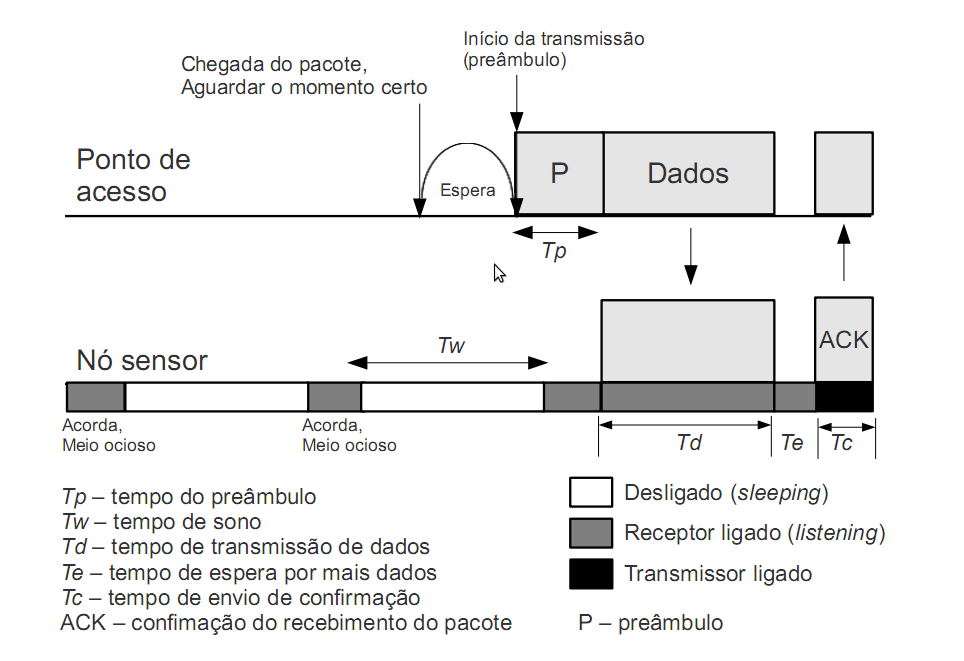
\includegraphics[width=340px,height=220px]{./Pictures/wisemac.png}
% SensorNodesScatteredInASensorField.png: 816x1056 pixel, 96dpi, 21.59x27.94 cm, bb=0 0 612 792
% pdfLaTeX aceita figuras no formato PNG, JPG ou PDF
% figuras vetoriais podem ser exportadas para eps e depois convertidas para pdf usando epstopdf
\caption{Funcionamento do WiseMAC \cite{El-Hoiydi2004}} %legenda
\label{fig:wisemac} %rotulo para refencia
\end{figure}

 \subsubsection{S-MAC}
 
 Sensor-MAC (S-MAC) [REF HERE] foi desenvolvido para ter primordialmente baixo consumo de energia, além disso conseguiu-se também boa escalabilidade e baixo número de colisões. Para conseguir esse resultados foram tratados os seguintes problemas identificados pelo autor como responsáveis pelo consumo excessivo de energia na rede: colisões de pacotes, que causam a retransmissão desses pacotes e consequente consumo extra de energia além de aumentar a latência na rede; \textit{overhearing}, que acontece quando os nós recebem pacotes que não são destinados a eles; excesso (\textit{overhead}) de pacotes de controle; e \textit{idle listening}, quando um nó permanece em modo de recepção aguardando por pacotes que não são enviados.

 Para alcançar esses resultados foi adotado um padrão ciclos de sono com períodos maiores de sono (nó desligado) e períodos de atividade curtos. Auto-organização está presente na sincronização dos períodos de atividade/sono dos nós em uma vizinhança, fazendo com que os nós adotem um mesmo cronograma de funcionamento. Isso possibilita que eles possam se comunicar e transmitir informações com eficiência apesar do maior tempo de inatividade. Além disso pode-se reduzir o tamanho dos preâmbulos%
 % PREÂMBULO 
 \footnote{Preâmbulo é um fluxo de dados utilizado para comunicar a intenção de transmitir. Tem duração variável de acordo com o período de sono, pois é preciso garantir que o destinatário receba esse preâmbulo e identifique-se como receptor dos pacotes de dados que serão enviados em seguida.}
 %
 pois tem-se uma garantia de que o(s) nó(s) aos quais os dados se destinam serão acordados no mesmo momento (ou em um momento muito próximo) em que aquele que deseja transmitir.
 
 Como desvantagem desse protocolo pode-se destacar que a sincronização dos ciclos de sono se dá entre um certo número de nós de uma região da rede e os nós que ficam no limiar entre duas regiões devem sincronizar-se com ambas as regiões (~\ref{fig:SmacSynch}). Isso faz com que o consumo de energia desses nós seja maior, reduzindo-se assim o seu tempo de vida útil.

\begin{figure}[!htb]
\centering
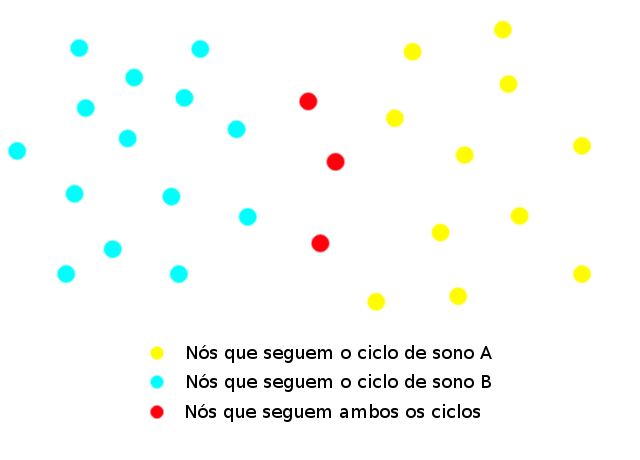
\includegraphics[width=290px,height=180px]{./Pictures/S-MACSynchronization.png}
% SensorNodesScatteredInASensorField.png: 816x1056 pixel, 96dpi, 21.59x27.94 cm, bb=0 0 612 792
% pdfLaTeX aceita figuras no formato PNG, JPG ou PDF
% figuras vetoriais podem ser exportadas para eps e depois convertidas para pdf usando epstopdf
\caption{Exemplo de sincronização de ciclos de atividades com protocolo S-MAC} %legenda
\label{fig:SmacSynch} %rotulo para refencia
\end{figure}
 
 
%\subsection{Transceiver operational states} \cite{Karl2005} pdf-p.47



% sensor-MAC (S-MAC), a MAC protocol
% explicitly designed for wireless sensor networks. While re-
% ducing energy consumption is the primary goal in our design,
% S-MAC also achieves good scalability and collision avoidance
% by utilizing a combined scheduling and contention scheme.
% To achieve the primary goal of energy efficiency, we need to
% identify what are the main sources that cause inefficient use of
% energy as well as what tradeoffs we can make to reduce energy
% consumption.
% 
% We have identified the following major sources of energy
% waste. The first one is collision. When a transmitted packet is
% corrupted, it has to be discarded, and follow-on re-transmis-
% sions increase energy consumption. Collision increases latency
% as well. The second source is overhearing, meaning that a
% node picks up packets that are destined to other nodes. The
% third source is control packet overhead. Sending and receiving
% control packets consumes energy too. The last major source of
% inefficiency is idle listening, i.e., listening to receive possible
% traffic that is not sent. This is especially true in many sensor
% network applications. If nothing is sensed, nodes are in idle
% mode for most of the time. 

%\subsection{Ciclos de Sono} 
 
%Com o objetivo de aumentar o tempo de vida útil das RSSF são utilizados ciclos de sono (\textit{sleep-wakeup cycle} ou \textit{duty cycle}) onde cada nó é ligado apenas por um curto período de tempo (\textit{wakeup}) e então desligado novamente (\textit{sleep}). Devido a utilização desse mecanismo, quando um nó precisa transmitir uma mensagem, ele deve permanecer ligado aguardando que seu destinatário também seja ligado e possa receber essa menságem. A utilização desse ciclos pode aumentar a vida útil das RSSF de poucos dias para vários meses ou mesmo anos dependendo da razão entre o tempo em que o nó permanece ligado e o tempo em que permanece desligado. Segundo \cite{1182838}, os parâmetros chave para caracterizar os ciclos de sono incluem tempo desligado(emph{sleep time}), tempo ligado(\textit{wakeup time}), e a energia consumida durante cada um dos estados (ligado/desligado). 
 
%Além da implementação de ciclos de sono também é possível utilizar ouros mecanismos para, em conjunto com ela, permitir um menor consumo de energia através da eliminação ou redução da ocorrência de outros problemas que podem ocasionar o consumo desnecessário de energia, como \textit{overhearing, protocol overhead, collision, idle lisetening, } etc. 
 
%Esse tipo de controle é realizado por protocolos MAC (Medium Access Control - Controle de Acesso ao Meio). Segundo Karl e Willing os protocolos MAC determinam para um nó os pontos no tempo quando ele pode acessar o meio para tentar trasmitir dados, controles ou pacotes de gerenciamento para outro nó (unicast) ou para um grupo de nós (multicast, broadcast). 
 